\chapter{Dezvoltarea aplicativ�}
\label{CapDA}

Absolventul va prezenta clar partea aplicativ� a lucr�rii �i metodologia de solu�ionare folosind elementele teoretice.

Se va specifica mediul de lucru, a facilit��ilor folosite �n acest mediu, proiectarea aplica�iei, detalii de implementare, exemple de test sau rezultate sub forma unor studii de caz, modul de utilizare a programului 
prin prezentarea documenta�iei de utilizare. Va fi anexat �n lucrare inclusive codul surs�.

Partea dezvolt�rii aplicative poate fi constituit� din mai multe capitole.

Referirea unei figuri \ref{Cap3Figura3-1}.

\begin{figure}[htbp]
	\centering
		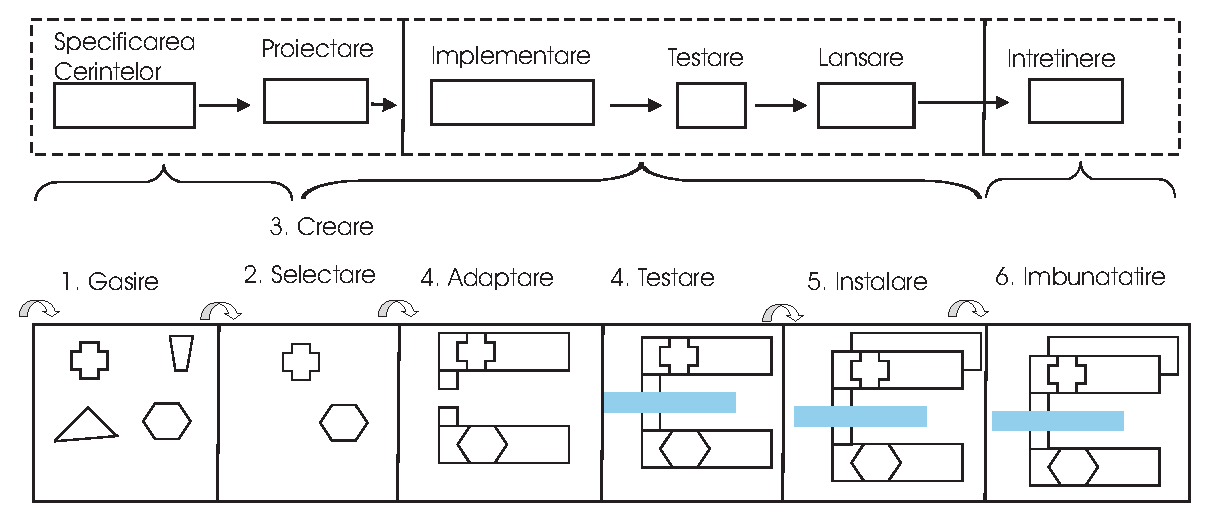
\includegraphics[scale=0.65]{Fig/fig_3_1.eps}
	\caption{Ciclul de dezvoltare al sistemelor bazate pe componente adaptat modelului cascad�}
	\label{Cap3Figura3-1}
\end{figure}


Referirea la Tabelul \ref{Cap3Tabel01}. 

\begin{table}[htbp]
\begin{center}
\begin{tabular}
{||p{100pt}||p{60pt}|p{60pt}||}
\hline
 Nume algoritm& 
 Toate solu�iile &
 Solu�ia optim�\\
\hline 
\hline Nume 1 & $20$ & $5$  \\
\hline Nume 2 & $20$ & $2$  \\
\hline
\end{tabular}
\end{center}
\caption{Solu�ii ob�inute }
\label{Cap3Tabel01}
\end{table}



\section{Prima sec�iune}

\subsection{Subsec�iunea unu}


Exemplu de prezentare algoritm.

\begin{algorithm}[htbp]
\begin{small}
\begin{algorithmic}  
\State \textbf{Input:}
\State {\ $\bullet$ the number $n$ ;}
\State {\ $\bullet$ the list $paramList$ of additional parameters that will be described in the proposed approaches.}
\State \textbf{Output:}
\State {\ $\bullet$ the solution.}
\State{}
\State {\textbf{Subalgorithm} \emph{IterativeBacktracking(n,[$paramListBack$])} is:}
\State \textbf{Begin}   
    \State {Let k := 1; possible[1] := \textit{init(1)};}   \Comment{initialise the search for the index k (=1)}
    \While {($k > 0$)}
    	\State {Let found := \textit{false}; v := possible[k];}
    	\While {( \textit{next(k,v,new)} \textbf{and} (not found))}
    			\State {Let v := new;}
    			\If {(\textit{conditionToContinue(k, possible,v,[$paramListCtC$])})}
    					\State { found := \textit{true};}
    			\EndIf    	
    	\EndWhile    
    	\If {(found)}
    			\State {Let possible[k] := v;}        \Comment{possible[1..k] is a solution candidate}
    			\If {(\textit{solution(n,k,possible,[$paramListSol$])})}          \Comment{found a solution}
    					\State {Print possible[1..k];}
    			\Else
    					\State { Let k := k+1;}     \Comment{step forward on level k+1}
    					\State {possible[k] := init(k);}
    			\EndIf    	
    	\Else
    			\State {k := k-1;}                 \Comment{step backward (backtrack to level k-1)}
    	\EndIf
    \EndWhile   
\State \textbf{End.}
\end{algorithmic}
\end{small}
\caption{The \textit{IterativeBacktracking} subalgorithm }
\label{AlgBackGeneral}
\end{algorithm}

\subsection{Subsec�iunea a doua}

\section{A doua sec�iune}

